%Start by an intuitive explanation of memory models. What it means for us and why was it introduced.
\section{Memory Consistency Models}

Concurrent programs take advantage of \textit{out-of-order} execution. 
Intuitively, this means that more than one unrelated computations can be done ``simultaneously'' without having any fixed order in which they should happen.
This results in concurrent programs having multiple different outcomes, the possible of which are described by a \textit{memory consistency model}. 

A lot of problems emerged with the introduction of concurrent computing. 
Starting with the famously known mutual exclusion problem way back in the 1960s introduced by Djikstra et al.~\cite{Djikstra} along with a solution, from it stemmed the ideas of semaphores and monitors that we all know today.  
Since then, a lot of well-known problems in concurrency such as The Producer Consumer Problem, Dining Philosopher's problem, Reader-Writer problem have come up, along with different algorithms to implement these in a practical sense, especially in Operating Systems. 

However, the above concerns in concurrency only revolved around the so-called "critical section"; which required that every thread trying to do something in a shared memory region must have exclusive access to it before doing anything. 
But as years went by, the need for more performance had increased, which also resulted in multiple hardwares having different features such as read-write buffers, caches, etc. 
Reliance on solely critical sections to perform operations on shared memory was observed as a bottleneck. 
Without its use, the possible outcomes of a concurrent program naturally increased.
The notion of \textit{atomicity} in actions done on shared memory became relatively unclear.  

\textit{Sequential Consistency}(SC), which was first formulated by Lamport et al.~\cite{Lamport79}, gives programmers a very intuitive way to reason about their programs running in a multiprocessor environment, especially without the use of critical sections.
SC guaranteed that every outcome of a program must be equivalent to a \textit{sequential interleaving} of each thread's individual actions. 
For example, consider the program in Figure~\ref{intro:Example} with two threads, which share memory denoted by $x$, $y$ initialized to 0, where $a$, $b$ are local variables. 
The right-hand-side are the possible values that $a$ and $b$ can read under sequential consistency rules.
%Show program 
\begin{figure}[H]
    \centering
    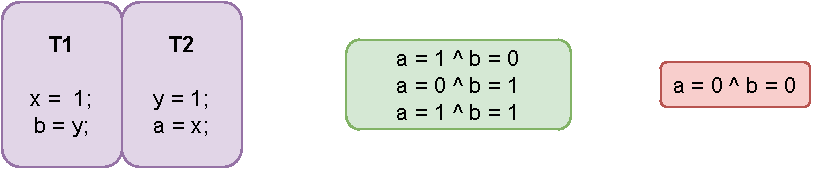
\includegraphics[scale=0.7]{2.Background/SC_Example1(a).pdf}
    \caption{Example program with its allowed and disallowed outcomes under SC.}
    \label{intro:Example}
\end{figure}

However, the above program under SC cannot have the outcome $a=0\ \wedge\ b=0$ as given in the red box to the right. 
To show that it is indeed not possible, assume that $a=0$. This means $x=1$ has not been done while $y=1$ has been done. 
This also means $b=y$ has not been done yet. 
Hence, if now the read to $y$ occurs, it cannot be $0$. The case is similar for when $b=0$. 
Such sequential reasoning though easy to understand and follow while writing concurrent programs, may not be that advantageous from a performance perspective.

From a program transformation perspective, \textit{Sequential Consistency} was also too ``strict'', in the sense that it may impede possible performance benefits of using low level optimization features, such as instruction reordering, elimination, introduction done by the hardware or at the compiler level.
A tutorial by Adve et al.~\cite{AdveG}, summarizes the most common hardware features for relaxed memory that are now available in most hardware. 
What this tutorial also exposed is the difficulty in formalizing such features in a way that we can reason about our programs sanely without getting caught up in the complexity of multiple executions of our programs. 
Such features relaxed the sequential reasoning in programs, and hence models describing their semantics came to be known as relaxed memory models.
Unsurprisingly, relaxed memory model specifications for different hardware/high level programming languages are still written in informal prose format, which lead to a number of problems in implementation~\cite{Sewell}. 
A position paper by Nardelli et al.~\cite{Nardelli} summarizes these problems well.
These informal specifications led to a number of inconsistencies in intention of the designer and how the programs behaved.

\paragraph{x86}
Intel's white paper on their earlier versions of the memory model for x86 was described in their white paper\cite{IntelW}.   
Sarkar et al.~\cite{SarkarS} showed that the then x86 model was fairly informal, which they formalize in their x86-CC memory model. 
Owens et al.~\cite{OwensS} later showed that the x86-CC model did not reflect precisely what x86 hardware intended, followed by exposing more problems in the latest specification of the x86 model given in the white paper of Intel \cite{IntelW}. 
They then propose a new model, x86-TSO as a remedy to this. The series of work in this exposed repeated inconsistencies between the specification and the implementation in hardware. 

While memory consistency models were initially only concerning hardware languages, as the years went by, even high level programming languages came up with their own memory models. 
This however, was not an easy process; several changes and edits are still made to memory models of Java and C11 to date, due to various new concerns about informal/ill-defined specifications that render the model useless for programmers to rely on. 

\paragraph{Java}
Pugh et al.~\cite{Pugh} showed the complexity of the initial versions of Java memory model, exposing with seemingly simplistic examples that even those involved in its inception were not sure about its specification. 
Later, Manson et al.~\cite{JeremyM} also exposed many limitations and under-specified semantics within the model, for which they proposed a new model with concise semantics. 
Manson et al.~\cite{Manson2} also concisely described the later version of the model, which had complex semantics to have \textit{out-of-thin-air} guarantees for programs with data-races. 
Recent works such as that done by Bender et al`.~\cite{BenderJ}, also showed us that the recent updates to the Java Memory model are still relatively unclear, which they again formalize. 

\paragraph{C++/C11}
Boehm et al.~\cite{Boehm} exposed that the earlier version of C++ concurrency semantics was unsound, followed by proposing a new semantics for the same.
Vafeiadis et al.~\cite{Vafeiadis2} summarized the open problems and verification results of the then version of C11 memory model. Some of these problems have been addressed, while some still remain open to date. 
Batty et al.~\cite{BattyM} exposed the lack of clear specifications of the then version of C11 memory model, giving a clarified, mathematical yet seemingly readable specification of the model.
Nienhuis et al.~\cite{Nienhuis} gave an operational semantics of the then C11 memory model, exposing certain limitations in terms of execution of such concurrent programs.
Lahav et al.~\cite{Lahav} exposed that the current compilation scheme of C11 concurrent programs to POWER unsound, thus proposing fixes to the memory model of C11 itself, which they call $RC11$.

\paragraph{Mixed-size models}
The above memory models were all based on the assumption that memory accesses are of equal sizes. 
But in practice, this may not always be the case. 
Hardware can have from 8-bit to 64-bit or event 128-bit memory accesses that can be done either atomically or split across different subsequent memory accesses. 
Investigation of semantics in this direction is fairly recent.
Flur et al.~\cite{Flur} investigated mixed-size behaviors in Arm and POWER architectures, also exposing new problems to address in the semantics. 
They also extend the current C11 memory model with some mixed-size semantics.
ECMAScript, being a relatively simpler mixed-size model has also had some attention in this respect. 
Watt et al~\cite{WattC} uncovered and fixed a deficiency in the previous version of the model, repairing the model to guarantee SC-DRF.
Our analysis is based on this corrected model which is incorporated in the ECMAScript draft specification. 
As far as our knowledge goes, no analysis has been done on this model to identify its implications on standard compiler optimizations. 


